\documentclass[12pt,a4paper]{article}
\usepackage{graphicx}
\usepackage{amsmath}
\begin{document}
\section{The exponential function}
The exponential function, commonly denoted as exp(x) or e\textsuperscript{x}, is a unique function of the form: \begin{equation}\label{eq:exponential form}
  f(x)=ab^x
\end{equation}
Where:
\begin{equation}\label{eq:exponential function}
  f(x)=e^x=ab^x,  a=1,b=2.71828...
\end{equation}
In this case the constant of proportionality is 1 and as such the differential of exp(x) is itself.
\begin{figure}[h]
  \centering
  \label{fig:exp}
  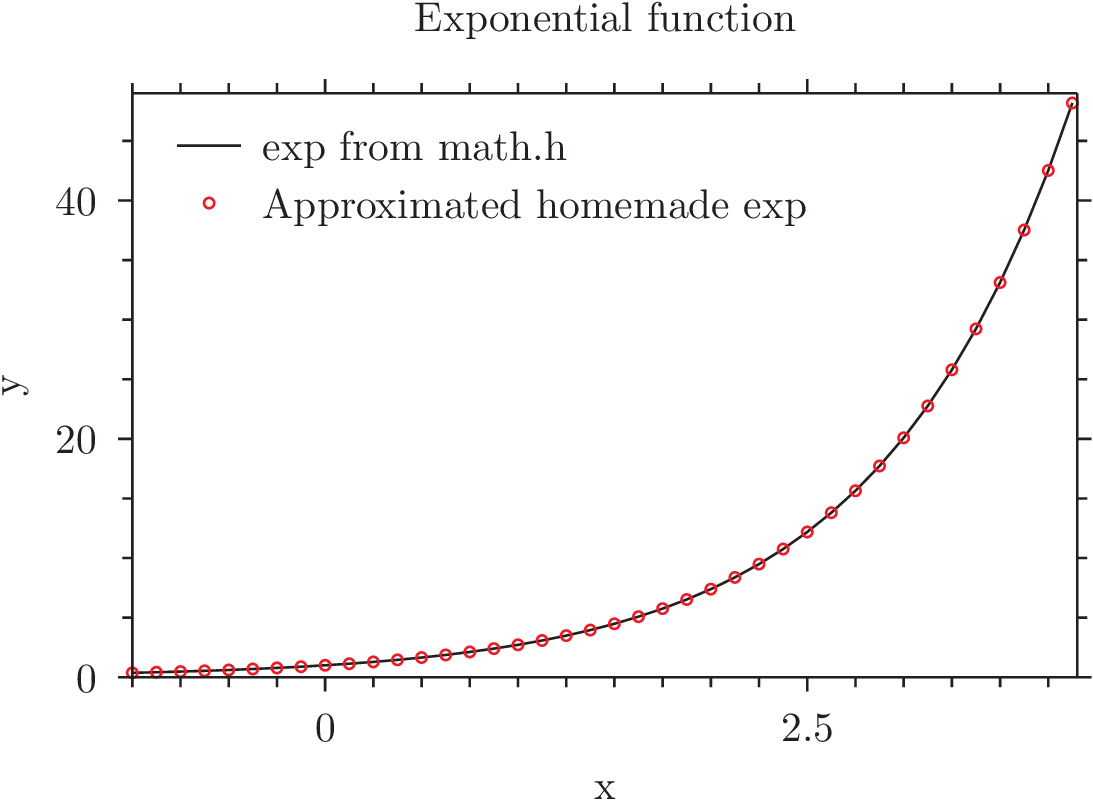
\includegraphics{exp.pyxplot.png}
  \caption{Exponential functions}
\end{figure}
\section{Implementation of exp}
The homemade implementation of the exponential function is ecpressed:\begin{multline}
  \label{eq:approx exp}
  exp(x)=1+x\times(1+\frac{x}{2}\times(1+\frac{x}{3}\times(1+\frac{x}{4}\times(1+\frac{x}{5}\times\\ (1+\frac{x}{6}\times(1+\frac{x}{7}\times(1+\frac{x}{8}\times(1+\frac{x}{9}\times(1+\frac{x}{10})))))))))
\end{multline}
Which is equivalent to the power series definition of the exponential function:
\begin{equation}
  \label{exp def}
  exp(x)=1+x+\frac{x^2}{2!}+\frac{x^3}{3!}+\frac{x^4}{4!}+...
\end{equation}
up to the tenth power. This can be easily seen by multiplying into the parentheses. The likeness of this implementation of the exponential function to the exponential function found in "math.h" can be observed in figure (\ref{fig:exp}). Defining the exponential function as equation (\ref{eq:approx exp}) has a specific advantage in numerical calculations as it does not include powers or factorials, making it less computationally intense.
\section{$exp(x)=exp(x/2)²$ approximation}
From equation (\ref{eq:exponential function}) we can see that for the classic exponential function that the $exp(x/2)²$ approximation holds as it is simply multiplying and dividing the exponent by 2, which cancels out. However for the implementation used in equation (\ref{eq:approx exp}) this only holds at low x as the Taylor expansion only holds at low x, therefore a condition is used: if $x>1/8$ return $exp(x/2)²$.
This condition ensures that only x'es where the approximation holds are used for the calculation of $exp(x)$.
\end{document}
